\documentclass[12pt, oneside]{amsart}   	% use "amsart" instead of "article" for AMSLaTeX format
\usepackage{geometry}                		% See geometry.pdf to learn the layout options. There are lots.
\geometry{letterpaper}                   		% ... or a4paper or a5paper or ... 
%\geometry{landscape}                		% Activate for for rotated page geometry
%\usepackage[parfill]{parskip}    		% Activate to begin paragraphs with an empty line rather than an indent
\usepackage{graphicx}				% Use pdf, png, jpg, or eps with pdflatex; use eps in DVI mode
								% TeX will automatically convert eps --> pdf in pdflatex		
\usepackage{amssymb}
\usepackage{amsmath}
\usepackage{subfig}
\usepackage{courier}
\newcommand{\us}{\textunderscore}

% for citing as (Mossong 2018)
\usepackage[round]{natbib}

% for underscore in urls
\usepackage{hyperref}

\usepackage{fullpage}

% to place table description above the table
\usepackage{float}
\floatstyle{plaintop}
\restylefloat{table}

% for pluscross sign
\usepackage{scalerel}

\title{COVID-19 Individual-Based Model  with Instantaneous Contract Tracing}
\author{Rob Hinch, Will Probert, Anel Nurtay, David Bonsall, Christophe Fraser} 
%\date{}							% Activate to display a given date or no date

\begin{document}
\maketitle
\tableofcontents

\section{Overview} \label{section_ibm_overview}
The individual-based model (IBM) is developed to simulate the spread of COVID-19 in a city and to analyse the effect of both passive and active intervention strategies.
It's primary purpose at this stage is to assist the design and evaluation of approaches to instantaneous contact tracing using an app that measures proximity events between phones with an app installed by phone users in the population.
The simulation will explore the effectiveness of the intervention using the app, based on the uptake of the app, on different ways of identifying index cases, different definitions of contact, different instructions to contacts.  
One of the main interventions for controlling an infection is testing of cases, and contact tracing to identify clusters of transmission. 
Contact tracing is difficult to model accurately in a simple mathematical model, and so an individual based simulation may be the most parsimonious way to accurately capture the effects of this intervention, especially when combined with other non-pharmaceutical interventions. 
The simulation was developed using parsimonious representations of the human contact network that is most relevant for a directly transmitted short generation time pathogen.
The simulation represents the three domains of interaction: the home; the workplace (or school for children, or regular social environment for older individuals); and the random interactions of daily life and travel.
The model is not spatially stratified at this stage.
The model is age stratified, as are the contact processes.
The contact processes are currently parameterised based on interviews of participants; it will be updated based on contact data collected by phone.  
The model of how the infection is spread via interactions between individuals is parameterised based on epidemiological studies of COVID-19 spread.
The disease process is currently modelled in only a basic manner that ensures that the time-scales of disease progression are correct. 
Since the impact of COVID-19 on hospitals is large, and the clinical outcome of infection depends on access to good hospital care, a more detailed models of patient flows and transmission within hospitals is planned. 

\section{Demographics}\label{section_ibm_demographics}

The demographics of the model are based upon UK national data for 2018 from the Office of National Statistics (ONS). 
For analyses of the infection spread within the population, individuals are categorised into nine groups by decades from age group (0-9 years) to (80+ years). 
The simulation is run on a static population and the proportion of individuals in each age group is the same as that specified by the population level statistics in Table~\ref{table_demographic_parameters}.
Every individual is part of a household which forms an important part of their daily interactions.
Household size data is shown in Table~\ref{table_demographic_parameters}.
Since the duration of the simulated epidemic is less than year, we do not consider changes in the population due to births, deaths due to other causes, and migration.

\begin{table}
\centering
\begin{tabular}{ |p{4cm}|p{7cm}|p{2cm}|  }
 \hline
 \multicolumn{3}{|c|}{Demographic Parameters} \\
 \hline
 Name   & Description & Value \\
 \hline
 \hline 
 \texttt{n\us total}    & Total population simulated  & 100,000  \\
\hline
\texttt{population\us 0\us 9}      & population 0-9 years old     & 8,052,552 \\
\texttt{population\us 10\us 19}    & population 10-19 years old   & 7,528,144 \\
\texttt{population\us 20\us 29}    & population 20-29 years old   & 8,711,750 \\
\texttt{population\us 30\us 39}    & population 30-39 years old   & 8,835,591 \\
\texttt{population\us 40\us 49}    & population 40-49 years old   & 8,715,439 \\
\texttt{population\us 50\us 59}    & population 50-59 years old   & 8,968,055 \\
\texttt{population\us 60\us 69}    & population 60-69 years old   & 7,069,544 \\
\texttt{population\us 70\us 79}    & population 70-79 years old   & 5,487,167 \\
\texttt{population\us 80}          & population 80+ years old     & 3,281,955 \\
 \hline 
\texttt{household\us size\us1} & households with 1 person (thousands) & 8,197 \\
\texttt{household\us size\us2} & households with 2 people (thousands) & 9,609 \\
\texttt{household\us size\us3} & households with 3 people (thousands) & 4,287 \\
\texttt{household\us size\us4} & households with 4 people (thousands) & 3,881 \\
\texttt{household\us size\us5} & households with 5 people (thousands) & 1,254 \\
\texttt{household\us size\us6} & households with 6 people (thousands) & 597 \\
 \hline
\end{tabular}
\caption{Age-stratified population of the UK and number of households containing $n$ people, with $n = 1, 2, \ldots 6$, provided by the ONS }
\label{table_demographic_parameters}
\medskip \medskip
\end{table}

\section{Interaction Network}\label{section_ibm_networks}

Every individual in the population is represented by a node in the simulation. 
Interactions between individuals are modelled via connections between nodes.
The connections form networks, which are generated to represent different types of daily interactions.
In this work we consider three types of networks that represent household, workplace, and miscellaneous interactions for the studied population.
Some of these networks are static and recur daily (e.g. household), whilst others are transient and are regenerated daily (e.g.  miscellaneous).
The interaction networks play two roles in the model, the first is that they can transmit the infection between individuals on each day that a connection is made.
Secondly, when we model contact-tracing via the phone app, the phone sees a subset of the network which is then used for contact-tracing.

The membership of different networks leads to age-group assortativity in the interactions.
A previous study of social contacts for infectious disease modelling has estimated the mean number of interactions that individuals have by age group~\citep{mossong2008social}.
This study is based on participants being asked to recall their interactions over the past day. 
We estimate mean interactions by age group by aggregating data (see Table~\ref{table_mean_daily_interactions}).
It is possible for an individual not to be connected to anybody (\emph{e.g.} a person living alone in a household).

%\medskip \medskip
\begin{table}
\centering
\begin{tabular}{ |p{5cm}|p{1.5cm}|  }
 \hline
 \multicolumn{2}{|c|}{Mean daily interactions} \\
 \hline
Age group  & Value \\
 \hline
 \hline 
children (0-19 years) & 15 \\
adults (20-69 years) & 13 \\
elderly (70+ years) & 7 \\
 \hline
\end{tabular}
\caption{Average number of interactions for an individual in each age group  acquired from empirical estimates~\citep{mossong2008social}}
\label{table_mean_daily_interactions}
\end{table}

\subsection{Household Network}\label{section_ibm_network_houshold}
Each individual is assigned to live in a single household.  
Each day every person has an interaction with everybody within their household.
The proportion of people living in households of different sizes is taken from ONS data (see~\nameref{section_ibm_demographics}).
So, for the population there are two important aggregate statistics that we match, the household-size structure and the population age-structure.
When individuals are assigned to households, we need to match both these aggregate statistics and also require that our households reflect typical age mixes.
To achieve this we used data for 125,455 households from the {\it Understanding Society} survey \citep{essex2019} containing household composition by age, which formed a reference household panel.
The household structure is then generated by sampling from the reference household panel with replacement.
To match the aggregate statistics for the population, we used a rejection-sampling method.
Households were sampled sequentially from the reference panel and accepted if combined with the existing samples the discrepancy with the target aggregate statistics was reduced.
If the discrepancy with the target aggregate statistics increased by less than a threshold, the new sample was still kept, otherwise it was rejected.
The threshold changes dynamically with each sample depending on whether it was accepted or rejected to keep a constant rejection rate throughout the sampling.
The discrepancy between the sample aggregate statistics and the target aggregate statistics was calculated by taking the sum of the square of the differences. 
Finally, we check the discrepancy of the total sampled set of households against the aggregate statistics and reject the whole sample if it is above a threshold.

\subsection{Work-place Networks}\label{section_ibm_network_workplace}
Each individual is a member of one work-place network. 
The work-place networks are modelled as Watts-Strogatz small-world networks~\citep{watts1998collective}.
When constructing the work-place networks, we assure the absence of overlaps between the household interactions and the local interactions on the small-world network.
Every day each person interacts with a random subset (50\%) of their connections on their work-place network.

For children, there are separate work-place networks for the both the 0y-9y age group (i.e. primary schools) and 10y-19y age groups (i.e secondary schools). 
On each of these networks we introduce a small number of adults (1 adult per 5 children) to represent teaching and other school staff.
Similarly for the 70y-79y age group and the 80y+ age group we have separate networks representing day-time social activities among elderly people (again with 1 adult per 5 elderly people).
All remaining adults (the vast majority) are part of the 20y-69y network.
Due to the difference in total number of daily interactions, each age group has a different number of interactions in their workplace network.
Parameters and values corresponding to the workplace network is shown in Table~\ref{table_work_place_network_parameters}.
Note the parameters are for the mean daily connections, so the number of interactions on the network are higher due to the daily sampling of connections.

\begin{table}
%\medskip \medskip
\centering
\resizebox{\textwidth}{!}{\begin{tabular}{|l|l|l|}
 \hline
 \multicolumn{3}{|c|}{Workplace Network Parameters} \\
 \hline
 Name   & Description & Value \\
 \hline
 \hline 
\texttt{mean\us work\us interaction\us child}    & mean daily connections on 0y-9y and 10y-19y networks & 10 \\
\texttt{mean\us work\us interaction\us adult}  & mean daily connections on the 20y-69y network & 7 \\
\texttt{mean\us work\us interaction\us elderly} & mean daily connections on the 70y-79y and 80y+ networks & 3 \\
\hline
\texttt{child\us network\us adults} & fraction of adults in child network & 0.2 \\
\texttt{elderly\us network\us adults} & fraction of adults in elderly network & 0.2 \\
\hline
\texttt{daily\us fraction\us work} & fraction of daily work connections made & 0.5 \\
\texttt{prob\us network\us rewire}$^*$ & rewiring probability of the  Watts-Stogatz small-world network & 0.1 \\ 
 \hline
\end{tabular}}
\caption{Mean numbers of daily connections for members of each age group, fraction of adults involved in occupational networks for children and for elderly people, and rewiring parameters for randomisation of daily interactions.}
\label{table_work_place_network_parameters}
\medskip \medskip
\end{table}

\subsection{Random Network}\label{section_ibm_network_random}
In addition to the recurring structured networks of households and workplaces, we include a number of random interactions as well.
These interactions occur once and are independent of the previous days connections.
The number of random connections an individual makes is the same each day (without interventions) and is drawn at the start of the simulation from a negative-binomial distribution, an over-dispersed skew distribution.
This variation in the number of interactions introduces ``super-spreaders'' into the network who have many more interactions than average.

\begin{table}
%\medskip \medskip
\centering
 \resizebox{\textwidth}{!}{\begin{tabular}{|l|l|l|}
 \hline
 \multicolumn{3}{|c|}{Random Network Parameters} \\
 \hline
 Name   & Description & Value \\
 \hline
 \hline 
\texttt{mean\us random\us interaction\us child}    & mean number of connections for children (0y-19y) & 2 \\
\texttt{mean\us random\us interaction\us adult}    & mean number of connections for adults (20y-69y) & 4 \\
\texttt{mean\us random\us interaction\us elderly} & mean number of connections for elderly (70y+) & 3 \\
\hline
\texttt{sd\us random\us interaction\us child}$^*$  & s.d.\ number of connections for children (0y-19y) & 2 \\
\texttt{sd\us random\us interaction\us adult}$^*$ & s.d.\ number of connections for adults (20y-69y) & 4 \\
\texttt{sd\us random\us interaction\us elderly}$^*$ & s.d.\ number of connections for elderly (70y+) & 3 \\
 \hline
\end{tabular}}
\caption{Parameters for numbers of random connections that members of each age group  have per day.}
\label{table_random_network_parameters}
\medskip \medskip
\end{table}

The mean numbers of connections were chosen so that the total number of daily interactions matched that from a previous study of social interaction~\citep{mossong2008social}. 
The number of random interactions was chosen to be lower in children in comparison to other age groups. 
In the simulation, each day a list is created containing all individuals who make random interactions and each person is repeated by the number of interactions they make.
This list is shuffled and interactions are made between adjacent pairs on the shuffled list.

\section{Infection Dynamics}\label{section_ibm_infection}
The infection is spread by interactions between infected and susceptible individuals. 
The rate of transmission is determined by three factors: the status of the infector, the age of the susceptible individual and the type of interaction (i.e.\ on which network did it occur).
We currently do not have data on the distribution of the length of interactions, so the effect of this on transmission is not modelled.

From early studies of COVID-19~\citep{ferretti2020quantifying, ganyani2020estimating} and
from similar infections~\citep{chan2003sars,anderson2004epidemiology,meltzer2004multiple}, we know that there is a delay between an individual becoming infected and when they become infectious.
The level of infectiousness increases with time and peaks roughly 4 days after the initial infection before decreasing.
Following~\citep{ferretti2020quantifying}, we model the infectiousness as a function of the length of time that the person has been infected for, which we model with a gamma function. 

It has been observed that some people who are infected with SARS-CoV-2 remain completely asymptomatic~\citep{bai2020presumed}, and we assume that these people are less infectious then those who go on to develop symptoms, a finding supported by the observation of lower viral load [Yang Liu et al Lancet  https://doi.org/10.1016/S1473-3099(20)30232-2]. 
Note, there is a difference between somebody who is asymptomatic (\emph{i.e.} who will never go on and develop symptoms), as opposed to somebody who is pre-symptomatic (\emph{i.e.} who will go on and develop symptoms at some point).
The term ``pre-symptomatic'' is used to describe people who are infectious while not having symptoms. 

The second factor that effects transmission is the susceptibility of the uninfected person. 
Data from China shows large differences in the number of infected individuals by age~\citep{chinavital}.
For example, the proportion of children infected is much lower than the proportion adults infected~\citep{lu2020sars}.
One explanation for fewer children being infected is that they are less susceptible than adults. 
Similarly, elderly people are more susceptible than adults due to accumulated predispositions. 
This dissimilarity between age groups is modelled by a multiplicative factor based upon the age group of the susceptible.

The third factor that we model is where the interaction took place (i.e.\ on which network).
Whilst we do not have data on the length of interactions, interactions which take place within a person's home will be closer than other types of interactions leading to higher rates of transmission.
This is modelled using a multiplicative factor.

Combining all effects, we model the rate at which the virus is transmitted in a single interaction by
\begin{equation}
\lambda(t,s_i,a_s,n) = \frac{R S_{a_s}A_{s_i} B_n}{ \bar I_{a_s}} \int_{t-1}^t f_{\Gamma}(u; \mu_i,\sigma_i^2) {\rm d}u,
\end{equation}
where $t$ is the time since infection; $s_i$ indicates whether the infector is asymptomatic; $a_s$ is the age to the susceptible; $n$ is the type of network where the interaction occurred; $\bar{I}_{a_s}$ is the mean number of daily interactions for somebody of the age of the susceptible; and $f_{\Gamma}(u; \mu,\sigma^2)$ is the p.d.f.\ of a gamma distribution.
With parameters: $R$ is the overall infectious rate; $S_{a_s}$ is the scale-factor for the age of the susceptible; $A_{s_i}$ is the scale-factor for the infector being asymptomatic; $B_n$ is the scale-factor for the network on which the interaction occurred; and, $\mu_i$ and $\sigma_i$ are the mean and width of the infectiousness curve.
Table~\ref{table_infectious_parameters} contains the values of the parameters used in simulations.
Note, that under some simplifying assumptions, $R$ becomes the basic reproduction number of the epidemic.
The rate of virus transmission is converted to a probability of transmission
\begin{equation}
P(t,s_i,a_s,n) = 1 - e^{-\lambda(t,s_i,a_s,n)}.
\end{equation}
The epidemic is seeded by infecting a number of individuals at the start of the infection.
The infection was assumed to take place on immediately before the simulation starts.

\medskip \medskip
\begin{table}
\centering
%\begin{tabular}{ |p{1.2cm}|p{6.8cm}|p{6.5cm}|p{1.2cm}|  }
\resizebox{\textwidth}{!}{\begin{tabular}{|l|l|l|l|}
 \hline
 \multicolumn{4}{|c|}{Infection Parameters} \\
 \hline
 Symbol & Name   & Description & Value \\
 \hline
 \hline 
$R$ & \texttt{infectious\us rate} & mean number of people infected by each infected person & $2.5^{\times}$ \\
$A_{\rm sym}$ &  - & relative infectious rate of symptomatic & 1 \\
$A_{\rm asym}$ & \texttt{asymptomatic\us infectious\us factor}& relative infectious rate of asymptomatic & $0.25$ \\
\hline
$B_{\rm home}$ & \texttt{relative\us transmission\us household}  & relative infectious rate of household interaction & $2$ \\
$B_{\rm work}$ & \texttt{relative\us transmission\us workplace}  & relative infectious rate of work interaction & $1$ \\
$B_{\rm random}$ & \texttt{relative\us transmission\us random}  & relative infectious rate of home interaction & $1$ \\
\hline
$S_{0-9}$ & \texttt{relative\us susceptibility\us 0\us 9} & relative susceptibility of age group 0 - 9 to an average person & $0.1^*$\\
$S_{10-19}$ & \texttt{relative\us susceptibility\us 10\us 19} & relative susceptibility of age group 10 - 19 to an average person  & $0.1^*$\\
$S_{20-29}$ & \texttt{relative\us susceptibility\us 20\us 29} & relative susceptibility of age group 20 - 29 to an average person  & $0.48^*$\\
$S_{30-39}$ & \texttt{relative\us susceptibility\us 30\us 39} & relative susceptibility of age group 30 - 39 to an average person  & $1.11^*$\\
$S_{40-49}$ & \texttt{relative\us susceptibility\us 40\us 49} & relative susceptibility of age group 40 - 49 to an average person  & $1.02^*$\\
$S_{50-59}$ & \texttt{relative\us susceptibility\us 50\us 59} & relative susceptibility of age group 50 - 59 to an average person  & $1.74^*$\\
$S_{60-69}$ & \texttt{relative\us susceptibility\us 60\us 69} & relative susceptibility of age group 60 - 69 to an average person & $2.34^*$\\
$S_{70-79}$ & \texttt{relative\us susceptibility\us 70\us 79} & relative susceptibility of age group 70 - 79 to an average person  & $2.03^*$\\
$S_{80}$ & \texttt{relative\us susceptibility\us 80} & relative susceptibility of age group 80+ to an average person & $2.24^*$\\
 \hline
 $\mu_i$ &  \texttt{mean\us infectious\us period} & time of peak infectiousness (i.e.\ the mean of the gamma p.d.f.) & $5^{\times}$  days\\
 $\sigma_i$ &  \texttt{sd\us infectious\us period} & width of infectiousness curve (i.e.\ the s.d.\ of the gamma p.d.f.) & $2^{\times}$ days\\
\hline
  -&  \texttt{n\us seed\us infection} & number of individual randomly infected at start of simulation & $10$ \\
 \hline

\end{tabular}}
\caption{Description of infection parameters and their values. Infectious rate and corresponding infectiousness parameters$^{\times}$ were obtained in Ref.~\citep{ferretti2020quantifying}. Relative values\protect{$^*$} are derived from the study of 44,672 confirmed patients in China~\protect{\citep{chinavital}} and are normalised with respect to the population of Hubei province from 2010. Number of infections in children\protect{$^\diamond$} include 171 cases from the report focused on patients of paediatric facility~\citep{lu2020sars}}
\label{table_infectious_parameters}
\end{table}
\medskip \medskip

\section{Natural history of infection}\label{section_ibm_disease}

Upon infection, an individual enters a disease progression cascade where the outcome and rates of progression depend on age of the infected person (see Figure~\ref{diseaseDynamics}).
The first split is that only a fraction of individuals develop symptoms ($1-\phi_{\rm asym}$), where a fraction ($\phi_{\rm asym}$) --- remain asymptomatic.
Those who are asymptomatic are infections (at a lower level, see~\nameref{section_ibm_infection} section) and will move to a recovered state after a time ($\tau_{\rm a,rec}$) drawn from a gamma distribution.
Once an individual is recovered we assume that they have immunity and cannot be reinfected.

Individuals, who are not asymptomatic, start by being in the pre-symptomatic state, where whilst they are be able to transmit the pathogen to others, they do not show any symptoms. 
This is important for modelling interventions because individuals in this state would not be able to self-isolate unless they had been contact-traced or there was a complete social distancing. 
After a time ($\tau_{\rm sym}$) drawn from a gamma distribution (the incubation period distribution), all pre-symptomatic individuals develop symptoms, at which point interventions can be triggered such as self-isolation, testing, and contact tracing.
Whilst most individuals will only develop mild symptoms, a fraction ($\phi_{\rm hosp}({\rm age})$) will go on to require hospitalisation, where the probability of requiring hospital treatment is age-dependent.
Those who do not require hospitalisation will recover after a time ($\tau_{\rm rec}$) drawn from a gamma distribution, whilst those who do --- enter hospital after a time ($\tau_{\rm hosp}$), which is drawn from a Bernoulli distribution of either 1 or 2 days.
Once entering hospital, a number of interventions can take place. 
We assume that a clinical diagnosis can immediately decide whether the patient is a case so that contract-tracing can be commenced straight away.
Of those who enter a hospital, a fraction ($\phi_{\rm crit}({\rm age})$) will become critical and require treatment in an ICU. 
The time from hospitalisation  to requiring critical care ($\tau_{\rm crit}$), is drawn from a Bernoulli distribution of either 1 or 2 days.
Finally, a fraction ($\phi_{\rm death}({\rm age})$)  of individuals who require critical care will die, with the time to death ($\tau_{\rm death}$) drawn from a gamma distribution.
Those who do not require critical care and those who do not die in critical care are assumed to recover after a time ($\tau_{\rm rec}$) drawn from a gamma distribution.

The disease state transitions are shown in Figure~\ref{diseaseDynamics} and the model parameters are in the table Disease Dynamics Parameters.

\begin{figure}
\centering
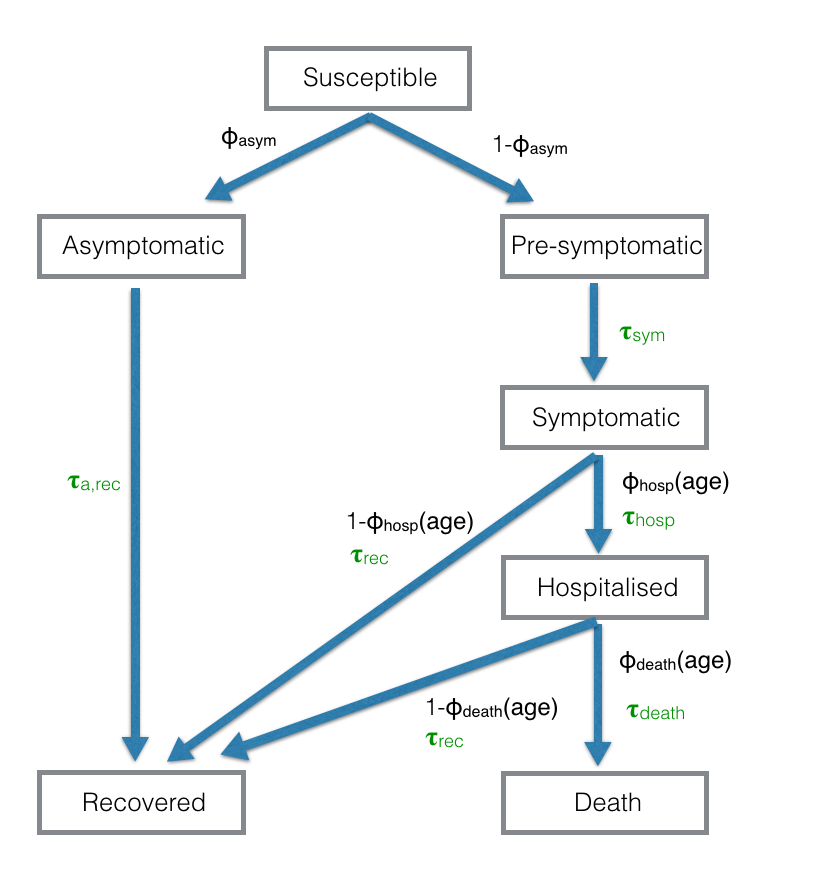
\includegraphics[width=.8\textwidth]{diseaseDynamics.png}
\caption{The disease status of an individual and the probability and time distribution of transitions. The $\phi_{\rm xxx}(\rm age)$ variables are the probability of transition to a particular state when there is a choice, where the probability depends upon the age of the individual.  The $\tau_{\rm xxx}$ are the gamma distributed variables of the time taken to make the transition.}
\label{diseaseDynamics}
\end{figure}

\medskip \medskip
\begin{table}
\centering
%\begin{tabular}{ |p{2.3cm}|p{6.4cm}|p{4cm}|p{1.4cm}|  }
\resizebox{\textwidth}{!}{\begin{tabular}{|l|l|l|l|l|}
 \hline
 \multicolumn{5}{|c|}{Disease Dynamics Parameters} \\
 \hline
 Symbol & Name  & Description & Value & Source \\
 \hline
 \hline 
  $\phi _{\rm asym} $  &  \texttt{fraction\us asymptomatic} & fraction of infected who are asymptomatic & 0.2 (0.179) & \citep{mizumoto2020estimating}\\
 \hline
$\phi_{\rm hosp}(0-9)$ & \texttt{hospitalised\us fraction\us 0\us 9} & fraction of hospitalisations among symptomatic age group 0 - 9 & $0.001$ & ~\citep{fergusonimpact}\\
$\phi_{\rm hosp}(10-19)$ & \texttt{hospitalised\us fraction\us 10\us 19} & fraction of hospitalisations among symptomatic age group 10 - 19 & $0.003$ & ~\citep{fergusonimpact}\\
$\phi_{\rm hosp}(20-29)$ & \texttt{hospitalised\us fraction\us 20\us 29} & fraction of hospitalisations among symptomatic age group 20 - 29  & $0.012$ & ~\citep{fergusonimpact}\\
$\phi_{\rm hosp}(30-39)$ & \texttt{hospitalised\us fraction\us 30\us 39} & fraction of hospitalisations among symptomatic age group 30 - 39  & $0.032$ & ~\citep{fergusonimpact}\\
$\phi_{\rm hosp}(40-49)$ & \texttt{hospitalised\us fraction\us 40\us 49} & fraction of hospitalisations among symptomatic age group 40 - 49 & $0.049$ & ~\citep{fergusonimpact}\\
$\phi_{\rm hosp}(50-59)$ & \texttt{hospitalised\us fraction\us 50\us 59} & fraction of hospitalisations among symptomatic age group 50 - 59 & $0.102$ & ~\citep{fergusonimpact}\\
$\phi_{\rm hosp}(60-69)$ & \texttt{hospitalised\us fraction\us 60\us 69} & fraction of hospitalisations among symptomatic age group 60 - 69 & $0.166$ & ~\citep{fergusonimpact}\\
$\phi_{\rm hosp}(70-79)$ & \texttt{hospitalised\us fraction\us 70\us 79} & fraction of hospitalisations among symptomatic age group 70 - 79 & $0.243$ & ~\citep{fergusonimpact}\\
$\phi_{\rm hosp}(80)$ & \texttt{hospitalised\us fraction\us 80} & fraction of hospitalisations among symptomatic age group 80+ & $0.273$ & ~\citep{fergusonimpact}\\
  \hline
$\phi_{\rm crit}(0-9)$ & \texttt{critical\us fraction\us 0\us 9} & fraction of hospitalised people in age group 0 - 9 in critical condition & $0.05$ & ~\citep{fergusonimpact}\\
$\phi_{\rm crit}(10-19)$ & \texttt{critical\us fraction\us 10\us 19} & fraction of hospitalised people in age group 10 - 19 in critical condition & $0.05$ & ~\citep{fergusonimpact}\\
$\phi_{\rm crit}(20-29)$ & \texttt{critical\us fraction\us 20\us 29} & fraction of hospitalised people in age group 20 - 29 in critical condition  & $0.05$ & ~\citep{fergusonimpact}\\
$\phi_{\rm crit}(30-39)$ & \texttt{critical\us fraction\us 30\us 39} & fraction of hospitalised people in age group 30 - 39 in critical condition  & $0.05$ & ~\citep{fergusonimpact}\\
$\phi_{\rm crit}(40-49)$ & \texttt{critical\us fraction\us 40\us 49} & fraction of hospitalised people in age group 40 - 49 in critical condition  & $0.63$ & ~\citep{fergusonimpact}\\
$\phi_{\rm crit}(50-59)$ & \texttt{critical\us fraction\us 50\us 59} & fraction of hospitalised people in age group 50 - 59 in critical condition & $0.122$ & ~\citep{fergusonimpact}\\
$\phi_{\rm crit}(60-69)$ & \texttt{critical\us fraction\us 60\us 69} & fraction of hospitalised people in age group 60 - 69 in critical condition & $0.274$ & ~\citep{fergusonimpact}\\
$\phi_{\rm crit}(70-79)$ & \texttt{critical\us fraction\us 70\us 79} & fraction of hospitalised people in age group 70 - 79 in critical condition & $0.432$ & ~\citep{fergusonimpact}\\
$\phi_{\rm crit}(80)$ & \texttt{fatality\us fraction\us 80} & fraction of hospitalised people in age group 80+ in critical condition & $0.709$ & ~\citep{fergusonimpact}\\
 \hline
$\phi_{\rm death}(0-9)$ & \texttt{fatality\us fraction\us 0\us 9} & fraction of fatalities among people in critical condition in age group 0 - 9 & $0.33$ & ~\citep{lu2020sars, dong2020epidemiological}\\
$\phi_{\rm death}(10-19)$  & \texttt{fatality\us fraction\us 10\us 19} & fraction of fatalities among people in critical condition in age group 10 - 19 & $0.25$ & ~\citep{lu2020sars, dong2020epidemiological}\\
$\phi_{\rm death}(20-29)$  & \texttt{fatality\us fraction\us 20\us 29} & fraction of fatalities among people in critical condition in age group 20 - 29  & $0.5$ & ~\citep{fergusonimpact}\\
$\phi_{\rm death}(30-39)$  & \texttt{fatality\us fraction\us 30\us 39} & fraction of fatalities among people in critical condition in age group 30 - 39  & $0.5$ & ~\citep{fergusonimpact}\\
$\phi_{\rm death}(40-49)$  & \texttt{fatality\us fraction\us 40\us 49} & fraction of fatalities among people in critical condition in age group 40 - 49 & $0.5$ & ~\citep{yang2020clinical}\\
$\phi_{\rm death}(50-59)$  & \texttt{fatality\us fraction\us 50\us 59} & fraction of fatalities among people in critical condition in age group 50 - 59 & $0.69$ & ~\citep{yang2020clinical}\\
$\phi_{\rm death}(60-69)$  & \texttt{fatality\us fraction\us 60\us 69} & fraction of fatalities among people in critical condition in age group 60 - 69 & $0.65$ & ~\citep{yang2020clinical}\\
$\phi_{\rm death}(70-79)$  & \texttt{fatality\us fraction\us 70\us 79} & fraction of fatalities among people in critical condition in age group 70 - 79 & $0.88$ & ~\citep{yang2020clinical}\\
$\phi_{\rm death}(80)$  & \texttt{fatality\us fraction\us 80} & fraction of fatalities among people in critical condition in  age group 80+ & $1$ & ~\citep{yang2020clinical}\\
 \hline
 \hline
$\mu_{\rm sym} $       &  \texttt{mean\us time\us to\us symptoms} & mean time to symptoms & 5.5 days & \citep{yang2020clinical}\\
$\sigma_{\rm sym} $  &  \texttt{sd\us time\us to\us symptoms}       & s.d.\ time to symptoms & 2.5 days & \citep{yang2020clinical}\\
 \hline
$\mu_{\rm hosp} $       &  \texttt{mean\us time\us to\us hospital}  & mean time to hospital after showing symptoms & 1.6 days & - \\
$\mu_{\rm crit} $       &  \texttt{mean\us time\us to\us critical}  & mean time to critical after hospitalisation & 1.5 days & - \\
 \hline
$\mu_{\rm death} $       &  \texttt{mean\us time\us to\us death} & mean time to death once hospitalised & 12 days & \citep{yang2020clinical} \\
$\sigma_{\rm death} $  &  \texttt{sd\us time\us to\us death}       & s.d.\ time to death once hospitalised & 5 days & \citep{yang2020clinical}\\
 \hline
$\mu_{\rm rec} $       &  \texttt{mean\us time\us to\us recover} & mean time to recover after symptoms/hospital &  12 days & \citep{yang2020clinical}\\
$\sigma_{\rm rec} $  &  \texttt{sd\us time\us to\us recover}       & s.d.\ time to recover after symptoms/hospital & 5 days & \citep{yang2020clinical}\\
 \hline
$\mu_{\rm a,rec} $       &  \texttt{mean\us asymptomatic\us to\us recover} & mean time to recover after asymptomatic &  15 days & \citep{yang2020clinical}\\
$\sigma_{\rm a,rec} $  &  \texttt{sd\us asymptomatic\us to\us recover}       & s.d.\ time to recover after asymptomatic & 5 days & \citep{yang2020clinical}\\
 \hline
\end{tabular}}
\caption{Proportion of people in each stage of illness whose disease progresses further; mean and standard deviation for density functions of the times that each transition -- disease progression or recovery -- takes}
\label{table_disease_dynamics_parmeters}
\end{table}

\section{Passive Interventions}\label{section_ibm_intervension_passive}

The model has the ability to model both passive and active interventions. 
Here we define an active intervention to be one involving testing or contact tracing with all other interventions being classed as passive.
Interventions are designed to reduce the rate of transmission, however, have the side-effect of potentially quarantining significant numbers of people. 

\subsection{Hospitalisation} Upon hospitalisation, a patient immediately stops interacting with both their household and workplace networks. We also reduce the number of random interactions that they have. An aspect of the disease transmission that we are missing in the model are the interactions within hospitals. 

\subsection{Self-Quarantine upon Symptoms} The next type of intervention we model is self-quarantine upon flu-like symptoms.
In addition to those infected by coronavirus, we infect a random a sample of the population each day with seasonal-flu which has similar symptoms. 
Upon experiencing symptoms, we put a fraction of patients in to self-quarantine immediately. 
Quarantine is modelled by not interacting with your workplace network and having a much reduced number of connections on your random network.
The length of quarantine is set to be up to 14 days, however, we model a fraction of the people dropping out of quarantine each day.
The simulation also contains the option that everybody in the household of a person with symptoms will also be asked to self-quarantine.


\begin{table}
\centering
\resizebox{\textwidth}{!}{
\begin{tabular}{|l|l|l|l|}
 \hline
 \multicolumn{3}{|c|}{Passive Intervention Parameters} \\
 \hline
 Name   & Description & Value \\
 \hline
\hline
\texttt{self\us quarantine\us fraction} & proportion of people who self quarantine upon symptoms &  0.8 \\
\texttt{quarantine\us household\us on\us symptoms}		&  quarantine household members of a person with a symptoms & 1 \\
\texttt{quarantine\us length\us self}  & maximum time of self-quarantined  & 14 days \\
\texttt{quarantine\us dropout\us self} & probability somebody drop out each day from self-quarantine & 0.01 \\
\texttt{quarantined\us daily\us interactions} & daily random interactions of a quarantined person &  0 \\
\texttt{hospitalised\us daily\us interactions} & daily random interactions of a hospitalised person &  0 \\
\texttt{seasonal\us flu\us rate} & daily probability of  seasonal flu &  0.0003  \\
 \hline
\end{tabular}}
\end{table}

\section{Active Interventions}\label{section_ibm_intervension_active}
We define active interventions as those which involve testing or actively tracing individuals in contact with an infected person (i.e.\ contact tracing).
There are 3 events in the model which can be the initial trigger for an active intervention:
\begin{enumerate}
    \item developing symptoms in the community
    \item testing positive for the infection
    \item hospitalisation with serious symptoms
\end{enumerate}
Note, for contract-tracing to occur, one of these events must be the initial trigger.
Along with being contact-traced, these are the key-times at which interventions can take place.
There are 3 types of active intervention which are
\begin{enumerate}
    \item testing for the infection
    \item request quarantining individuals (i.e. at home)
    \item notifying contacts via the app 
\end{enumerate}
\subsection{Testing} Currently the test for coronavirus is not sensitive immediately upon infection, which we model by only returning a positive test if the patient has been infected for 3 days when the test takes place. 
For individuals who are already displaying symptoms this is not an issue since the symptoms normally only present after the test has become sensitive. 
However, when ordering a test for somebody who has been contact-traced, we assume that the positive individual is the source of the infection and delay testing until the test would be sensitive. Currently there are also delays in the testing procedure, both in taking a test and in getting the result for it. 
These test delays are modelled which will then delay further interventions thus reducing their efficacy.

\subsection{Request Quarantining} 
Individuals can be requested to quarantine themselves at home upon receiving a positive test or being contact-traced. 
The request for quarantine is set to be 14 days, with a daily random dropout of people leaving quarantine early. 
This rate of dropout depends upon the reason the person was asked to self-quarantine, which models the fact that people who have received a positive test results are more likely to honour the full quarantine period then those who are only traced.

\subsection{App-based Contact Tracing} 
The third intervention we model is the app-based contract-tracing, which can initiate the quarantining of infected individuals prior to them ever showing symptoms. 
For infections with high levels of pre-symptomatic transmission this is vital to control epidemics. 
Contact tracing can only originate from somebody with the app and can only trace others who have the app as well. 
Given that the whole population will not have the app, we randomly pick a fraction of the population to not have the app. 
Secondly, the app is likely to miss some interactions between individuals, even if both individuals have the app, so when contact-tracing we randomly drop a number of interactions. 
To contact-trace we go through all the interactions the individual has had for the past 5 days where both parties have the app and the interaction has not been missed, and send a message to the contact.
This message can ask the individual to quarantine themselves, be tested and trigger further contact-tracing.
\medskip

We now go through the 3 initial trigger events and the event of being contract-traced and describe the intervention options we (optionally) model.

\subsection{On flu-like symptoms} We have already described how some people will self-quarantine when they display symptoms. 
However, there is also an intervention option to order a test for person who has flu-like symptoms. 
This allows us to find confirmed cases of the virus in the community, which will act as a trigger for contact-tracing.

\subsection{On positive-test} 
When an individual has received a positive test, we can request that they self-quarantine (normally they are already self-quarantining, but a positive test should make them be more likely to stick out the full 14 days).
The next policy option is to ask for the household members of the person with the positive test to self-quarantine as well.
We can then reach beyond the household by using the app to send a message to all the reachable contacts of the person who tested positive.
Additionally there is the option to send a message to all the reachable contacts of everybody in the household of the person who tested positive. 

\subsection{On hospitalisation} 
When an individual enters hospital with suspected COVID-19 a test is ordered to confirm the diagnosis. 
However, at this point the model contains the option for a clinical diagnosis of COVID-19 by a hospital doctor to be made, which can immediate set off the policy options that a positve-test would.
This allows contact-tracing to be initiated much more rapidly than waiting for a test, which improves the efficacy of the intervention.

\subsection{On contact-traced} 
When an individual has been contact-traced, we can ask them to self-quarantine.
There is also the option for asking all the household members of the person who has been traced to self-quarantine.
Once somebody has been traced as being suspected of being infected, we can order a test for this person. 
There are a couple of reasons for wanting to do this. 
First, a positive test will make the person more likely to self-quarantine for the full requested period and also allow other treatment and care pathways to be initiated (especially important for vulnerable people).
Secondly, a confirmed positive test can trigger further rounds of contact-tracing via the app.
This type of recursion requires a positive-test at each level and prevents large number of people being  quarantined following a single positive result.
A different type of recursion via the app is to immediately trace the contacts of those traced following the original positive-test (i.e. second degree contacts on the network). 
This dramatically increases the number of people who are quarantined from a single positive-test, however, this will quarantine more people who are infected earlier giving the opportunity to prevent the epidemic spreading further.
The key difference between these types of recursion is the delay caused by testing. 
If testing could be carried out quickly, then you could test at each round of recursion and still catch the front of the epidemic.

\begin{table}
\centering
\resizebox{\textwidth}{!}{\begin{tabular}{|l|l|l|}
 \hline
 \multicolumn{3}{|c|}{Active Intervention Parameters} \\
 \hline
 Name   & Description & Value \\
 \hline
 \hline
\texttt{app\us users\us fraction} & fraction of population with the app & 0.85 \\
\texttt{quarantine\us days} & the number of days prior contacts to contact & 5 days \\
\texttt{traceable\us interaction\us raction} & fraction of interactions that captured if both users have app & 0.8 \\
\texttt{tracing\us network\us depth} & depth of interaction network to contact (i.e.\ second-order contacts) & 1 \\
\hline
\hline
\texttt{quarantine\us on\us traced} & quarantine individuals who are traced & 1 \\
\texttt{test\us on\us traced}            & test individuals who have been contact-traced & 1 \\
\texttt{test\us on\us symptoms}      & test individuals who show symptoms and are quarantined & 1 \\
\texttt{allow\us clinical\us diagnosis} & commence contact tracing on a hospital clinical diagnosis & 1 \\
\hline
\hline
\texttt{quarantine\us household\us on\us positive}	& quarantine household members of a person with a positive test & 1\\
\texttt{quarantine\us household\us on\us traced}		&  quarantine household members of a person who has been traced  & 1\\
\texttt{quarantine\us household\us contacts\us on\us positive}	& quarantine the contacts of each household member of a person who tests positive & 1\\	
\hline
\hline
\texttt{quarantine\us length\us traced}     & maximum time of quarantined if traced  & 14 days \\
\texttt{quarantine\us dropout\us traced}   & probability somebody drop out each day if traced  & 0.01 \\
\texttt{quarantine\us length\us positive}   & maximum time of quarantine if test positive & 14 days \\
\texttt{quarantine\us dropout\us positive} & probability somebody drop out each day if tested positve & 0.01 \\
\hline
\hline
\texttt{test\us insensitive\us period} & number of days following infection the test is insensitive & 3 days\\
\texttt{test\us order\us wait} & minimum number of days to wait to take a test  & 1 days \\
\texttt{test\us result\us wait} & number of days to wait for a test result & 1 days \\
 \hline 
\end{tabular}}
\end{table}


\section{Implementation Details}\label{section_ibm_implementation}
This is a high-level description of how the model is implemented.
The model is coded in C but using an object-orientated pattern.
All required memory is pre-allocated at the start of the simulation for efficiency.

\subsection{Events} \label{section_ibm_implementation_events}
We use an event-based system to drive disease progression in individuals and interventions, where at each decision point we calculate when the next event will occur and add it to an event-list for that day.
For each type of event there is an \texttt{eventlist} structure, which contains an array of linked-lists for each day of the simulation.
We use doubly-linked lists to allow for efficient deletion as well as insertion of events.
Event-lists also keep track of the current and total number of events by type (defined as all entries today and in the past). 

\subsection{Individuals} \label{section_ibm_implementation_individuals}
Each person in the population is represented by an \texttt{individual} structure and the population is static.
The \texttt{individual} structure contains the following information:
\begin{enumerate}
\item Demographic - age, house number, network membership
\item Interaction diary - list of all interactions over a period of days (note this is not only the ones tracked by the app)
\item Disease - current status (i.e.\ symptomatic) and pointers to both current and future disease events
\item Quarantine - is the person currently quarantined and pointers to that event and the release event
\end{enumerate}

\subsection{Network Construction}\label{section_ibm_implementation_network}
Each interaction network has an associated \texttt{network} structure which contains an array of edges.
Network structures can be static (i.e.\ household), static but down-sampled (i.e.\ workplace) or dynamically generated at each time step (i.e.\ random).
Network generation is modular and any network can be added to the model as long as it can be represented by an array of edges.
Once all the networks have been defined, we add each edge to the individuals interaction diary (which are single-linked lists as deletion is not required).

\subsection{Infectious transmission}\label{section_ibm_implementation_disease}
The next step is to transmit the pathogen across today's interaction network, which is done as push from all infected people (by disease status).
For every infectious status, we pre-calculate the transmission rate for someone who has been infected for that length of time.
At each time-step, we go through all that interactions the infected person had for that day and calculate whether transmission has occurred.
Instead of randomly drawing whether transmission has occurred for each interaction, we allocate each individual a quantity of {\it hazard} (from an exponential distribution) at the start of the simulation.
Each interaction with an infected person reduces the persons {\it hazard} and when a person's {\it hazard} drops below 0 they become infected. 
This is mathematically equivalent to randomly drawing individual interactions, which can be seen by calculating the probability of  being infected by the $N^{\rm th}$ interaction  $P({\rm infected} \  N^{\rm th})$, after exposured to interactions with hazard-rates $\{ \lambda_1,..,\lambda_N \}$
\begin{align*}
P({\rm infected} \  N^{\rm th}) 
&= P_N \prod_{i=1}^{N-1} ( 1 - P_i) \\
&= \exp\left( -\sum_{i=1}^{N-1} \lambda_i \right) - \exp\left( -\sum_{i=1}^{N} \ \lambda_i\right) \\
&= P \left(  \sum_{i=1}^{N-1} \lambda_i  < T <  \sum_{i=1}^{N} \lambda_i \right)
\end{align*}
where $T$ is distributed exponentially with mean 1. 
The fact that different age groups have a different susceptibilities ($S_{a_s}$) is then modelled by allocating different amounts of initial {\it hazard} to each group.
This improves computational efficiency so that is it not necessary to draw a random variable for each potential transmission event.

\subsection{Performance} The model for 100k individuals takes approximately 100ms per day to run and requires 250Mb of memory on a 2015 MacBook Pro. 
Both speed and memory are linear in population size (tested from 100k to 1m). 
96\% of the CPU usage is spent on rebuilding the daily interaction networks and updating the individual's interaction diaries.
About 60\% of the memory usage is spent on storing the interaction diaries (for 5 days), another 20\% is spent on storing the semi-static networks with the remaining 20\% spent on storing individuals and their states in event-lists.


\newpage
%\section{References}
\renewcommand{\bibname}{References}
\bibliographystyle{abbrvnat}
\bibliography{lib} 
\end{document}  


